\documentclass[a4paper, 12pt]{article}

%\usepackage{cmap}
\usepackage[T2A]{fontenc}
\usepackage[utf8]{inputenc}
\usepackage[english, russian]{babel}
\usepackage{graphicx}
\usepackage[top=1in, bottom=1in, left=3.2cm, right=2.6cm]{geometry}
\graphicspath{./}
\usepackage{biblatex}
\addbibresource{lib.bib}
\linespread{1.5}
\usepackage{ragged2e}
\justifying
\usepackage{listings}
\usepackage{color}


\begin{document}
	
\begin{titlepage}
	\fontsize{12pt}{12pt}\selectfont
	\begin{figure}[t!]
		\centering
		
\includegraphics[scale=0.8]{bmstu}
	\end{figure}
	
	\noindent\rule{15cm}{3pt}
	\newline\newline
	\noindent 
	ФАКУЛЬТЕТ 
	\underline{«Информатика и системы управления»} \newline\newline
	
	\noindent КАФЕДРА \underline{«Программное обеспечение ЭВМ и информационные технологии»}\newline\newline\newline\newline\newline
	
	\centering {\Large Отчет по лабораторной работе № 3}
	\vspace{1mm}
	
	\centering {\Large По курсу: "Функциональное и логическое программирование"
		\vspace{8mm}	
		
		\centering \bf Работа интерпретатора Lisp.}
	\vspace{8mm}
	
	
	\begin{flushright}
		{\small	Студент:\\ Турсунов Жасурбек Рустамович \\ Группа: ИУ7-56Б
			\vspace{3mm}
			\\Преподователи: \\ Толпинская Наталья Борисовна \\ Строганов Юрий Владимирович}
	\end{flushright}
	
	\begin{center}
		\vfill
		Москва, \the\year
		~г.
	\end{center}
\end{titlepage}

\tableofcontents
\clearpage
\newpage

\textbf{Цель работы:} приобрести навыки работы в системе Common Lisp.
\\ \hspace*{5mm} \textbf{Задачи работы:} изучить работу интерпретатора Lisp, алгоритм работы функции eval, структуру и порядок обработки программы в Lisp.


\section*{Введение}
\addcontentsline{toc}{section}{Введение}

\hspace*{5mm} Программа на Lisp представляет собой вызов функции на верхнем уровне. Функции в Lisp делятся на типичные(математические) функции и формы - функции, которые особым образом обрабатывают свои аргументы, то есть требуют специальной обработки. Кроме того, функции в Lisp носят частичный характер, то есть по разному, иногда не корректно работают на множестве S-выражений.
\\ \hspace*{5mm} Синтаксически программа оформляется в виде S-выражения (обычно - списка). S-выражение, попавшее на вход системы анализирует функция eval. S-выражение очень часто может быть структурированным.
\clearpage
\newpage

\section*{Задание 1}
\addcontentsline{toc}{section}{Задание 1}
Составить диаграмму вычисления следующих выражений:\\

\hspace*{40mm}\begin{tabular}{ | l | l | }
	\hline
	\textbf{Выражение} & \textbf{Результат} \\ \hline
	(equal 3 (abs -3)) & T \\ \hline
	(equal (+ 1 2) 3) & T \\ \hline
	(equal (* 4 7) 21) & Nil \\ \hline
	(equal (* 2 3) (+ 7 2)) & Nil \\ \hline
	(equal (- 7 3) (* 3 2)) & Nil \\ \hline
	(equal (abs (- 2 4)) 3) & Nil \\ \hline
\end{tabular}
\begin{figure}[h!]
	\centering 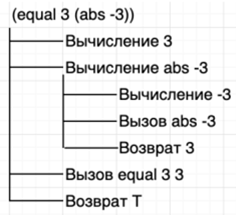
\includegraphics[scale=2.5]{1}
	\centering\caption{(equal 3 (abs -3))}
\end{figure}
\begin{figure}[h!]
	\centering 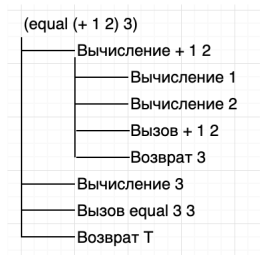
\includegraphics[scale=2.5]{2}
	\centering\caption{(equal (+ 1 2) 3)}
\end{figure}
\clearpage
\newpage
\begin{figure}[h!]
	\centering 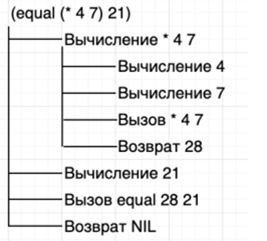
\includegraphics[scale=2.5]{3}
	\centering\caption{(equal (* 4 7) 21)}
\end{figure}
\begin{figure}[h!]
	\centering 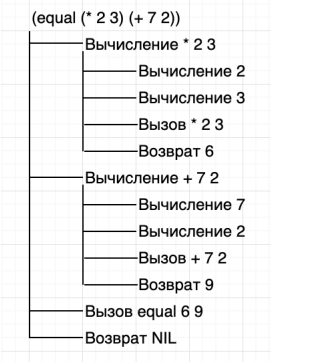
\includegraphics[scale=2.5]{4}
	\centering\caption{(equal (* 2 3) (+ 7 2))}
\end{figure}
\clearpage
\newpage
\begin{figure}[h!]
	\centering 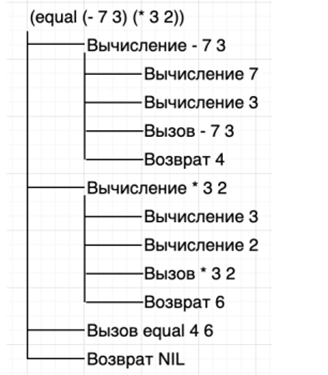
\includegraphics[scale=2.5]{5}
	\centering\caption{(equal (- 7 3) (* 3 2))}
\end{figure}
\begin{figure}[h!]
	\centering 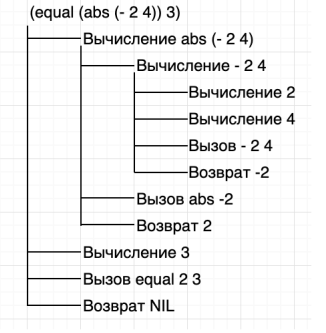
\includegraphics[scale=2.5]{6}
	\centering\caption{(equal (abs (- 2 4)) 3)}
\end{figure}


\section*{Задание 2}
\addcontentsline{toc}{section}{Задание 2}
Написать функцию, вычисляющую гипотенузу прямоугольного треугольника по заданным катетам и составить диаграмму её вычисления.
\definecolor{codegreen}{rgb}{0,0.6,0}
\definecolor{codegray}{rgb}{0.5,0.5,0.5}
\definecolor{codepurple}{rgb}{0.58,0,0.82}
\definecolor{backcolour}{rgb}{0.95,0.95,0.92}

\lstdefinestyle{mystyle}{
	backgroundcolor=\color{backcolour},   
	commentstyle=\color{codegreen},
	keywordstyle=\color{magenta},
	numberstyle=\tiny\color{codegray},
	stringstyle=\color{codepurple},
	basicstyle=\ttfamily\footnotesize,
	breakatwhitespace=false,         
	breaklines=false,                 
	captionpos=b,                    
	keepspaces=true,                 
	numbers=left,                    
	numbersep=5pt,                  
	showspaces=false,                
	showstringspaces=false,
	showtabs=false,                  
	tabsize=4
}

\lstset{style=mystyle}
\begin{lstlisting}
	(defun hyp (k1 k2)
			(sqrt (+ (* k1 k1) (* k2 k2)))
	)
\end{lstlisting}
\begin{figure}[h!]
	\centering 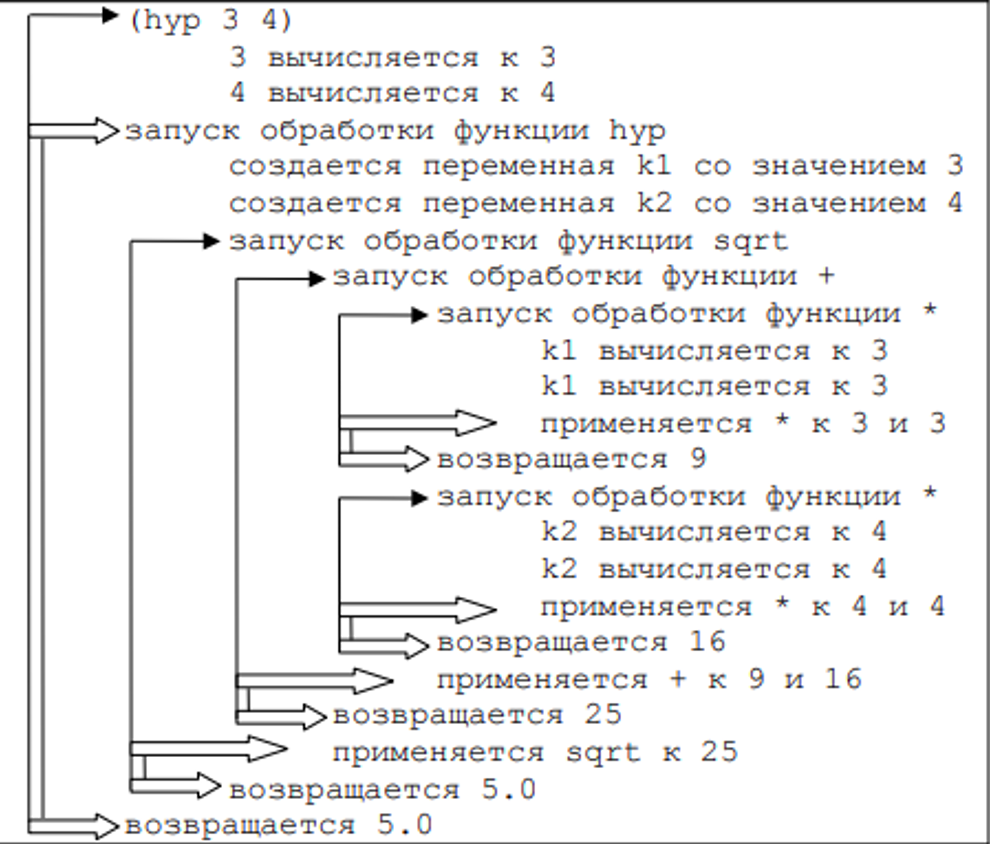
\includegraphics[scale=1]{hyp}
	\centering\caption{диаграмма функции вычисляющую гипотенузу треугольника}
\end{figure}

\section*{Задание 3}
\addcontentsline{toc}{section}{Задание 3}
Написать функцию, вычисляющую объем параллелепипеда по 3-м его сторонам,  и составить диаграмму ее вычисления.
\begin{lstlisting}
	(defun volume (a b c)
			(* a b c)
	)
\end{lstlisting}
\clearpage
\newpage
\begin{figure}[h!]
	\centering 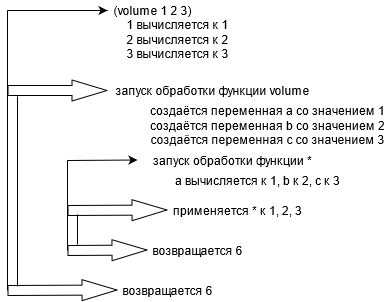
\includegraphics[scale=0.8]{vol}
	\centering\caption{диаграмма функции вычисляющую объем параллелепипеда}
\end{figure}

\section*{Задание 4}
\addcontentsline{toc}{section}{Задание 4}
Каковы результаты вычисления следующих выражений?\\ \\
\hspace*{20mm}\begin{tabular}{ | l | l | }
	\hline
	\textbf{Выражение} & \textbf{Результат} \\ \hline
	(list 'a 'b 'c) & (A B C) \\ \hline
	(cons 'a (b c)) & undefined function: B \\ \hline
	(cons 'a '(b c)) & (A B C) \\ \hline
	(caddr (1 2 3 4 5)) & illegal function call \\ \hline
	(cons 'a 'b 'c) & invalid number of arguments \\ \hline
	(list 'a (b c)) & the variable C is unbound \\ \hline
	(list a '(b c)) & the variable A is unbound \\ \hline
	(list (+ 1 '(length '(1 2 3)))) & (length '(1 2 3)) is not type of number \\ \hline
\end{tabular}
\\ \\ Пояснения:
\begin{enumerate}
	\item \textbf{the variable C is unbound} – возникает при попытке получить значение символа не связанного со значением;
	\item \textbf{undefined function: B} – не была определена вызываемая функция;
	\item \textbf{invalid number of arguments} - в функцию было передано неверное количество аргументов;
	\item \textbf{illegal function call} -возникает при попытке в качестве имени функции передать не символ.
\end{enumerate}

\section*{Задание 5}
\addcontentsline{toc}{section}{Задание 5}
Напишите функцию longer\_than от двух списков аргументов, которая возвращает Т, если первый аргумент имеет большую длину. Проверьте работу функции на одноуровневом и структурированном списке.\\
\begin{lstlisting}
	(defun longer_then (a b)
			(> (length a) (length b))
	)
\end{lstlisting}
\hspace*{20mm}\begin{tabular}{ | l | l | }
	\hline
	\textbf{Выражение} & \textbf{Результат} \\ \hline
	(longer\_than '(1 2 3) '(1 2)) & T \\ \hline
	(longer\_than '(1 (2 (3 (4)))) '(1 (2 (3)))) & Nil \\ \hline
\end{tabular}


\section*{Задание 6}
\addcontentsline{toc}{section}{Задание 6}
Каковы результаты вычисления следующих выражений?\\ \\
\hspace*{10mm}\begin{tabular}{ | l | l | }
	\hline
	\textbf{Выражение} & \textbf{Результат} \\ \hline
	(cons 3 (list 5 6)) & (3 5 6) \\ \hline
	(cons 3 '(list 5 6)) & (3 LIST 5 6) \\ \hline
	(list 3 'from 9 'gives (- 9 3)) & (3 FROM 9 GIVES 6) \\ \hline
	(+ (length '(1 foo 2 too)) (car '(21 22 23))) & 25 \\ \hline
	(cdr '(cons is short for ans)) & (IS SHORT FOR ANS) \\ \hline
	(car (list one two)) & the variable ONE is unbound \\ \hline
	(car (list 'one 'two)) & ONE \\ \hline
\end{tabular}
\clearpage
\newpage
Пояснения:
\begin{enumerate}
	\item \textbf{the variable ONE is unbound} – возникает при попытке получить значение символа не связанного со значением.
\end{enumerate}

\section*{Ответы на вопросы:}
\addcontentsline{toc}{section}{Ответы на вопросы}
\hspace*{-7mm} \textbf{1) Базис Lisp:}

\hspace*{-6mm}Базис - это минимально необходимый набор конструкций с помощью которого можно запрограммировать. Базис Lisp образуют атомы, структуры, базовые функции, базовые функционалы

\hspace*{-13mm} \textbf{2) Классификация функций:}
\begin{enumerate}
	\item базовые функции:
		\begin{enumerate}
			\item селекторы (car, cdr);
			\item конструкторы(cons);
			\item предикаты (atom, Null, lisp, ..);
			\item функции сравнения (eq, eql, =, equal, equalp).
		\end{enumerate}
	\item формы;
	\item функционалы.
\end{enumerate}
\hspace*{-8mm} \textbf{3) Представление и интерпретация списков}
\\Списки представлены с помощью списковых ячеек. В списковой ячейке хранится двауказателя: на голову и хвост. Способ интерпретации определяется положением выражения и алгоритмом функционирования Лисп-системы. 
\\\hspace*{-8mm} \textbf{4) Функции CAR и CDR}
\\CAR и CDR являются базовыми функциями доступа к данным. CAR принимает точечную пару или пустой список в качестве аргумента и возвращает первый элемент или nil, соответственно. CDR принимает точечную  пару или пустой список и возвращает список состоящий из всех элементов, кроме первого. Если в списке меньше двух элементов, то возвращается Nil.
\\\hspace*{-8mm} \textbf{5) Назначение и отличие в работе Cons и List}
\\ List и Cons являются функциями создания списков (Cons–базовая, List–нет).Функция Cons создает списочную  ячейку  и  устанавливает два указателя на аргументы. Функция List принимает переменное число аргументов и возвращает список, элементы которого – переданные в функцию аргументы.

\end{document}